
%% This style is provided exclusively for the ICSE 2012 main conference,
%% ICSE 2012 co-located events, and ICSE 2012 workshops.

%% bare_conf_ICSE12.tex
%% V1.4
%% 2012-01-21
%%

%% This is a skeleton file demonstrating the use of IEEEtran.cls
%% (requires IEEEtran.cls version 1.7 or later) with an IEEE conference paper.
%%
%% Support sites:
%% http://www.michaelshell.org/tex/ieeetran/
%% http://www.ctan.org/tex-archive/macros/latex/contrib/IEEEtran/
%% and
%% http://www.ieee.org/

%%*************************************************************************
%% Legal Notice:
%% This code is offered as-is without any warranty either expressed or
%% implied; without even the implied warranty of MERCHANTABILITY or
%% FITNESS FOR A PARTICULAR PURPOSE! 
%% User assumes all risk.
%% In no event shall IEEE or any contributor to this code be liable for
%% any damages or losses, including, but not limited to, incidental,
%% consequential, or any other damages, resulting from the use or misuse
%% of any information contained here.
%%
%% All comments are the opinions of their respective authors and are not
%% necessarily endorsed by the IEEE.
%%
%% This work is distributed under the LaTeX Project Public License (LPPL)
%% ( http://www.latex-project.org/ ) version 1.3, and may be freely used,
%% distributed and modified. A copy of the LPPL, version 1.3, is included
%% in the base LaTeX documentation of all distributions of LaTeX released
%% 2003/12/01 or later.
%% Retain all contribution notices and credits.
%% ** Modified files should be clearly indicated as such, including  **
%% ** renaming them and changing author support contact information. **
%%
%% File list of work: IEEEtran.cls, IEEEtran_HOWTO.pdf, bare_adv.tex,
%%                    bare_conf.tex, bare_jrnl.tex, bare_jrnl_compsoc.tex
%%*************************************************************************

% *** Authors should verify (and, if needed, correct) their LaTeX system  ***
% *** with the testflow diagnostic prior to trusting their LaTeX platform ***
% *** with production work. IEEE's font choices can trigger bugs that do  ***
% *** not appear when using other class files.                            ***
% The testflow support page is at:
% http://www.michaelshell.org/tex/testflow/



% Note that the a4paper option is mainly intended so that authors in
% countries using A4 can easily print to A4 and see how their papers will
% look in print - the typesetting of the document will not typically be
% affected with changes in paper size (but the bottom and side margins will).
% Use the testflow package mentioned above to verify correct handling of
% both paper sizes by the user's LaTeX system.
%
% Also note that the "draftcls" or "draftclsnofoot", not "draft", option
% should be used if it is desired that the figures are to be displayed in
% draft mode.
%
\documentclass[10pt, conference, compsocconf]{IEEEtran}
% Add the compsocconf option for Computer Society conferences.
%
% If IEEEtran.cls has not been installed into the LaTeX system files,
% manually specify the path to it like:
% \documentclass[conference]{../sty/IEEEtran}

\usepackage{graphicx,amssymb,amstext,amsmath}
\usepackage{balance}
\usepackage{hyperref}
\usepackage{multirow}


% Some very useful LaTeX packages include:
% (uncomment the ones you want to load)


% *** MISC UTILITY PACKAGES ***
%
%\usepackage{ifpdf}
% Heiko Oberdiek's ifpdf.sty is very useful if you need conditional
% compilation based on whether the output is pdf or dvi.
% usage:
% \ifpdf
%   % pdf code
% \else
%   % dvi code
% \fi
% The latest version of ifpdf.sty can be obtained from:
% http://www.ctan.org/tex-archive/macros/latex/contrib/oberdiek/
% Also, note that IEEEtran.cls V1.7 and later provides a builtin
% \ifCLASSINFOpdf conditional that works the same way.
% When switching from latex to pdflatex and vice-versa, the compiler may
% have to be run twice to clear warning/error messages.






% *** CITATION PACKAGES ***
%
%\usepackage{cite}
% cite.sty was written by Donald Arseneau
% V1.6 and later of IEEEtran pre-defines the format of the cite.sty package
% \cite{} output to follow that of IEEE. Loading the cite package will
% result in citation numbers being automatically sorted and properly
% "compressed/ranged". e.g., [1], [9], [2], [7], [5], [6] without using
% cite.sty will become [1], [2], [5]--[7], [9] using cite.sty. cite.sty's
% \cite will automatically add leading space, if needed. Use cite.sty's
% noadjust option (cite.sty V3.8 and later) if you want to turn this off.
% cite.sty is already installed on most LaTeX systems. Be sure and use
% version 4.0 (2003-05-27) and later if using hyperref.sty. cite.sty does
% not currently provide for hyperlinked citations.
% The latest version can be obtained at:
% http://www.ctan.org/tex-archive/macros/latex/contrib/cite/
% The documentation is contained in the cite.sty file itself.






% *** GRAPHICS RELATED PACKAGES ***
%
\ifCLASSINFOpdf
  % \usepackage[pdftex]{graphicx}
  % declare the path(s) where your graphic files are
  % \graphicspath{{../pdf/}{../jpeg/}}
  % and their extensions so you won't have to specify these with
  % every instance of \includegraphics
  % \DeclareGraphicsExtensions{.pdf,.jpeg,.png}
\else
  % or other class option (dvipsone, dvipdf, if not using dvips). graphicx
  % will default to the driver specified in the system graphics.cfg if no
  % driver is specified.
  % \usepackage[dvips]{graphicx}
  % declare the path(s) where your graphic files are
  % \graphicspath{{../eps/}}
  % and their extensions so you won't have to specify these with
  % every instance of \includegraphics
  % \DeclareGraphicsExtensions{.eps}
\fi
% graphicx was written by David Carlisle and Sebastian Rahtz. It is
% required if you want graphics, photos, etc. graphicx.sty is already
% installed on most LaTeX systems. The latest version and documentation can
% be obtained at: 
% http://www.ctan.org/tex-archive/macros/latex/required/graphics/
% Another good source of documentation is "Using Imported Graphics in
% LaTeX2e" by Keith Reckdahl which can be found as epslatex.ps or
% epslatex.pdf at: http://www.ctan.org/tex-archive/info/
%
% latex, and pdflatex in dvi mode, support graphics in encapsulated
% postscript (.eps) format. pdflatex in pdf mode supports graphics
% in .pdf, .jpeg, .png and .mps (metapost) formats. Users should ensure
% that all non-photo figures use a vector format (.eps, .pdf, .mps) and
% not a bitmapped formats (.jpeg, .png). IEEE frowns on bitmapped formats
% which can result in "jaggedy"/blurry rendering of lines and letters as
% well as large increases in file sizes.
%
% You can find documentation about the pdfTeX application at:
% http://www.tug.org/applications/pdftex





% *** MATH PACKAGES ***
%
%\usepackage[cmex10]{amsmath}
% A popular package from the American Mathematical Society that provides
% many useful and powerful commands for dealing with mathematics. If using
% it, be sure to load this package with the cmex10 option to ensure that
% only type 1 fonts will utilized at all point sizes. Without this option,
% it is possible that some math symbols, particularly those within
% footnotes, will be rendered in bitmap form which will result in a
% document that can not be IEEE Xplore compliant!
%
% Also, note that the amsmath package sets \interdisplaylinepenalty to 10000
% thus preventing page breaks from occurring within multiline equations. Use:
%\interdisplaylinepenalty=2500
% after loading amsmath to restore such page breaks as IEEEtran.cls normally
% does. amsmath.sty is already installed on most LaTeX systems. The latest
% version and documentation can be obtained at:
% http://www.ctan.org/tex-archive/macros/latex/required/amslatex/math/





% *** SPECIALIZED LIST PACKAGES ***
%
%\usepackage{algorithmic}
% algorithmic.sty was written by Peter Williams and Rogerio Brito.
% This package provides an algorithmic environment fo describing algorithms.
% You can use the algorithmic environment in-text or within a figure
% environment to provide for a floating algorithm. Do NOT use the algorithm
% floating environment provided by algorithm.sty (by the same authors) or
% algorithm2e.sty (by Christophe Fiorio) as IEEE does not use dedicated
% algorithm float types and packages that provide these will not provide
% correct IEEE style captions. The latest version and documentation of
% algorithmic.sty can be obtained at:
% http://www.ctan.org/tex-archive/macros/latex/contrib/algorithms/
% There is also a support site at:
% http://algorithms.berlios.de/index.html
% Also of interest may be the (relatively newer and more customizable)
% algorithmicx.sty package by Szasz Janos:
% http://www.ctan.org/tex-archive/macros/latex/contrib/algorithmicx/




% *** ALIGNMENT PACKAGES ***
%
%\usepackage{array}
% Frank Mittelbach's and David Carlisle's array.sty patches and improves
% the standard LaTeX2e array and tabular environments to provide better
% appearance and additional user controls. As the default LaTeX2e table
% generation code is lacking to the point of almost being broken with
% respect to the quality of the end results, all users are strongly
% advised to use an enhanced (at the very least that provided by array.sty)
% set of table tools. array.sty is already installed on most systems. The
% latest version and documentation can be obtained at:
% http://www.ctan.org/tex-archive/macros/latex/required/tools/


%\usepackage{mdwmath}
%\usepackage{mdwtab}
% Also highly recommended is Mark Wooding's extremely powerful MDW tools,
% especially mdwmath.sty and mdwtab.sty which are used to format equations
% and tables, respectively. The MDWtools set is already installed on most
% LaTeX systems. The lastest version and documentation is available at:
% http://www.ctan.org/tex-archive/macros/latex/contrib/mdwtools/


% IEEEtran contains the IEEEeqnarray family of commands that can be used to
% generate multiline equations as well as matrices, tables, etc., of high
% quality.


%\usepackage{eqparbox}
% Also of notable interest is Scott Pakin's eqparbox package for creating
% (automatically sized) equal width boxes - aka "natural width parboxes".
% Available at:
% http://www.ctan.org/tex-archive/macros/latex/contrib/eqparbox/





% *** SUBFIGURE PACKAGES ***
%\usepackage[tight,footnotesize]{subfigure}
% subfigure.sty was written by Steven Douglas Cochran. This package makes it
% easy to put subfigures in your figures. e.g., "Figure 1a and 1b". For IEEE
% work, it is a good idea to load it with the tight package option to reduce
% the amount of white space around the subfigures. subfigure.sty is already
% installed on most LaTeX systems. The latest version and documentation can
% be obtained at:
% http://www.ctan.org/tex-archive/obsolete/macros/latex/contrib/subfigure/
% subfigure.sty has been superceeded by subfig.sty.



%\usepackage[caption=false]{caption}
%\usepackage[font=footnotesize]{subfig}
% subfig.sty, also written by Steven Douglas Cochran, is the modern
% replacement for subfigure.sty. However, subfig.sty requires and
% automatically loads Axel Sommerfeldt's caption.sty which will override
% IEEEtran.cls handling of captions and this will result in nonIEEE style
% figure/table captions. To prevent this problem, be sure and preload
% caption.sty with its "caption=false" package option. This is will preserve
% IEEEtran.cls handing of captions. Version 1.3 (2005/06/28) and later 
% (recommended due to many improvements over 1.2) of subfig.sty supports
% the caption=false option directly:
%\usepackage[caption=false,font=footnotesize]{subfig}
%
% The latest version and documentation can be obtained at:
% http://www.ctan.org/tex-archive/macros/latex/contrib/subfig/
% The latest version and documentation of caption.sty can be obtained at:
% http://www.ctan.org/tex-archive/macros/latex/contrib/caption/




% *** FLOAT PACKAGES ***
%
%\usepackage{fixltx2e}
% fixltx2e, the successor to the earlier fix2col.sty, was written by
% Frank Mittelbach and David Carlisle. This package corrects a few problems
% in the LaTeX2e kernel, the most notable of which is that in current
% LaTeX2e releases, the ordering of single and double column floats is not
% guaranteed to be preserved. Thus, an unpatched LaTeX2e can allow a
% single column figure to be placed prior to an earlier double column
% figure. The latest version and documentation can be found at:
% http://www.ctan.org/tex-archive/macros/latex/base/



%\usepackage{stfloats}
% stfloats.sty was written by Sigitas Tolusis. This package gives LaTeX2e
% the ability to do double column floats at the bottom of the page as well
% as the top. (e.g., "\begin{figure*}[!b]" is not normally possible in
% LaTeX2e). It also provides a command:
%\fnbelowfloat
% to enable the placement of footnotes below bottom floats (the standard
% LaTeX2e kernel puts them above bottom floats). This is an invasive package
% which rewrites many portions of the LaTeX2e float routines. It may not work
% with other packages that modify the LaTeX2e float routines. The latest
% version and documentation can be obtained at:
% http://www.ctan.org/tex-archive/macros/latex/contrib/sttools/
% Documentation is contained in the stfloats.sty comments as well as in the
% presfull.pdf file. Do not use the stfloats baselinefloat ability as IEEE
% does not allow \baselineskip to stretch. Authors submitting work to the
% IEEE should note that IEEE rarely uses double column equations and
% that authors should try to avoid such use. Do not be tempted to use the
% cuted.sty or midfloat.sty packages (also by Sigitas Tolusis) as IEEE does
% not format its papers in such ways.





% *** PDF, URL AND HYPERLINK PACKAGES ***
%
%\usepackage{url}
% url.sty was written by Donald Arseneau. It provides better support for
% handling and breaking URLs. url.sty is already installed on most LaTeX
% systems. The latest version can be obtained at:
% http://www.ctan.org/tex-archive/macros/latex/contrib/misc/
% Read the url.sty source comments for usage information. Basically,
% \url{my_url_here}.





% *** Do not adjust lengths that control margins, column widths, etc. ***
% *** Do not use packages that alter fonts (such as pslatex).         ***
% There should be no need to do such things with IEEEtran.cls V1.6 and later.
% (Unless specifically asked to do so by the journal or conference you plan
% to submit to, of course. )


% correct bad hyphenation here
\hyphenation{op-tical net-works semi-conduc-tor}


\begin{document}
%
% paper title
% can use linebreaks \\ within to get better formatting as desired
\title{Fragmentation: A Comparison of Android Vendor's Bugs via Topic Analysis}


% author names and affiliations
% use a multiple column layout for up to two different
% affiliations

\author{\IEEEauthorblockN{Dan Han, Chenlei Zhang, Xiaochao Fan, Abram Hindle, Kenny Wong, Eleni Stroulia}
\IEEEauthorblockA{Department of Computing Science\\
University of Alberta \\
Edmonton, Canada\\
\{dhan3, chenlei1, xf2, hindle1, kenw, stroulia\}@cs.ualberta.ca}

}

% conference papers do not typically use \thanks and this command
% is locked out in conference mode. If really needed, such as for
% the acknowledgment of grants, issue a \IEEEoverridecommandlockouts
% after \documentclass

% for over three affiliations, or if they all won't fit within the width
% of the page, use this alternative format:
% 
%\author{\IEEEauthorblockN{Michael Shell\IEEEauthorrefmark{1},
%Homer Simpson\IEEEauthorrefmark{2},
%James Kirk\IEEEauthorrefmark{3}, 
%Montgomery Scott\IEEEauthorrefmark{3} and
%Eldon Tyrell\IEEEauthorrefmark{4}}
%\IEEEauthorblockA{\IEEEauthorrefmark{1}School of Electrical and Computer Engineering\\
%Georgia Institute of Technology,
%Atlanta, Georgia 30332--0250\\ Email: see http://www.michaelshell.org/contact.html}
%\IEEEauthorblockA{\IEEEauthorrefmark{2}Twentieth Century Fox, Springfield, USA\\
%Email: homer@thesimpsons.com}
%\IEEEauthorblockA{\IEEEauthorrefmark{3}Starfleet Academy, San Francisco, California 96678-2391\\
%Telephone: (800) 555--1212, Fax: (888) 555--1212}
%\IEEEauthorblockA{\IEEEauthorrefmark{4}Tyrell Inc., 123 Replicant Street, Los Angeles, California 90210--4321}}




% use for special paper notices
%\IEEEspecialpapernotice{(Invited Paper)}




% make the title area
\maketitle


\begin{abstract}
Android fragmentation has been a controversial topic, but both proponents and opponents cannot provide strong evidences to support their statements. In order to make the debate more clear, we mined and analyzed the Android bug reports related to two popular Android vendors, HTC and Motorola. We manually annotated bug reports with labels and applied Labeled Latent Dirichlet Allocation (LDA) to the datasets to produce bug topics. By comparing the average relevance of top 20 bug topics over time for both vendors, we categorized the topics into two types which are common topics and unique topics. We investigated and discussed these two types of bug topics relevance tendency over time. Our analysis results lead to the conclusion that Android fragments into multiple incompatible and brand-specific versions. Our findings can be used by Android system community, stakeholders, Android device vendors and developers to make project dashboards, process investigation and feature analysis.

\end{abstract}

\begin{IEEEkeywords}
Bug reports; Topic mining; Labeled LDA
\end{IEEEkeywords}


% For peer review papers, you can put extra information on the cover
% page as needed:
% \ifCLASSOPTIONpeerreview
% \begin{center} \bfseries EDICS Category: 3-BBND \end{center}
% \fi
%
% For peerreview papers, this IEEEtran command inserts a page break and
% creates the second title. It will be ignored for other modes.
\IEEEpeerreviewmaketitle



\section{Introduction}
% no \IEEEPARstart
The market share of mobile phones is always increasing and getting more and more competitive among various mobile device vendors\footnote{\url{http://asymco.com/2011/11/17/the-global-smartphone-market-landscape}}. iPhone and Android phone share the majority of mobile device market. Compared to Apple’s closed ecosystem for iOS, Android system has many fragmentation. These fragmentation highlights include Android five major versions, diverse customized Android versions and various Android mobile devices provided by different device vendors \cite{androidfragmentation}.

Android fragmentation has been a controversial topic which swells up now and again. Some people argue that there should be many issues about the fragmentation on Android platform. They hold the point that there are too many existing Android versions, various Android mobile devices running these versions and too many branches from multiple vendors \cite{androidfragmentation}\cite{timetoendfragmentation}. On the other hand, there is an opposite viewpoint that there is no issues about fragmentation in Android community, only differentiation \cite{androidcompatibility}. However, both proponents and opponents cannot provide strong evidences to support their statements.

In order to make this debate more clear, we will explore the bug topics for different vendors from Android bug reports using Labeled LDA [1]. We choose the bug reports of HTC and Motorola in this study. HTC’s first Android phone was the HTC Dream manufactured in Oct. 2008. HTC has made more than thirty different Android phones since then. Motorola made their first Android phone in Oct. 2009 and has released more than twenty different Android phones since then . Their Android products have gained widespread popularity. 

In this study, our goal is to investigate the topics in bug reports related to the two Android vendors, HTC and Motorola, with the purpose of understanding how their bug topics evolve over time.  We utilize the Labeled LDA, a novel technique in software engineering, to build the topic models and analyze the topic evolution models\cite{Thomas:2010} of bug reports in HTC and Motorola. Researchers have applied LDA and other topic models to a lot of software projects\cite{Marcus04aninformation}\cite{Asuncion:2010}\cite{Linstead:2009}\cite{Thomas:2011}. We will also apply LDA on our data and try to evaluate the performance between LDA and Labeled LDA.

This paper makes the following contributions:

\begin{itemize}
\item We introduce the Labeled LDA to build topic models.
\end{itemize}

\begin{itemize}
\item We empirically compare the performance of LDA and Labeled LDA on the bug reports of HTC and Motorola.
\end{itemize}

\begin{itemize}
\item We analyze the topic evolution models in Android platform for HTC and Motorola by mining their bug reports.
\end{itemize}

\begin{itemize}
\item Our findings support that Android community does have fragmentation issues.
\end{itemize}

The paper is organized as follows: Section 2 describes the background; we discuss the related work in section 3; in section 4, we explicate our methodology about the mining approaches applied on this study; section 5 is to compare and evaluate the topic models generated by LDA and Labeled LDA; we introduce the analysis of topic evolution models in section 6; the paper concludes with a discussion of two research questions, threats to validity, conclusion and future work in section 7, 8 and 9 correspondingly. 

% You must have at least 2 lines in the paragraph with the drop letter
% (should never be an issue)

%\subsection{Subsection Heading Here}
%Subsection text here.


%\subsubsection{Subsubsection Heading Here}
%Subsubsection text here.

\section{Background}
In our research, we apply Labeled LDA to perform topic analysis. Labeled LDA is a supervised topic model for credit attribution in multi-labeled corpora\cite{labeledlda}. It defines a one-to-one mapping between LDA’s latent topics and tags labeled by users. In other words, Labeled LDA incorporates the multiple tags into the topics learning process and only builds topics around these tags, which is quite different from LDA. LDA, as a totally unsupervised algorithm, automatically learns a set of terms for each topic on a corpus without any constraints. To apply Labeled LDA, we utilize the Stanford Topic Modeling Toolbox (STMT)\cite{stmt}. Specifically, this tool outputs a set of topics, each one consisting of a list of terms, and the relevance distribution between each bug report and all the topics.


%\begin{figure*}[htb]
%\centering
%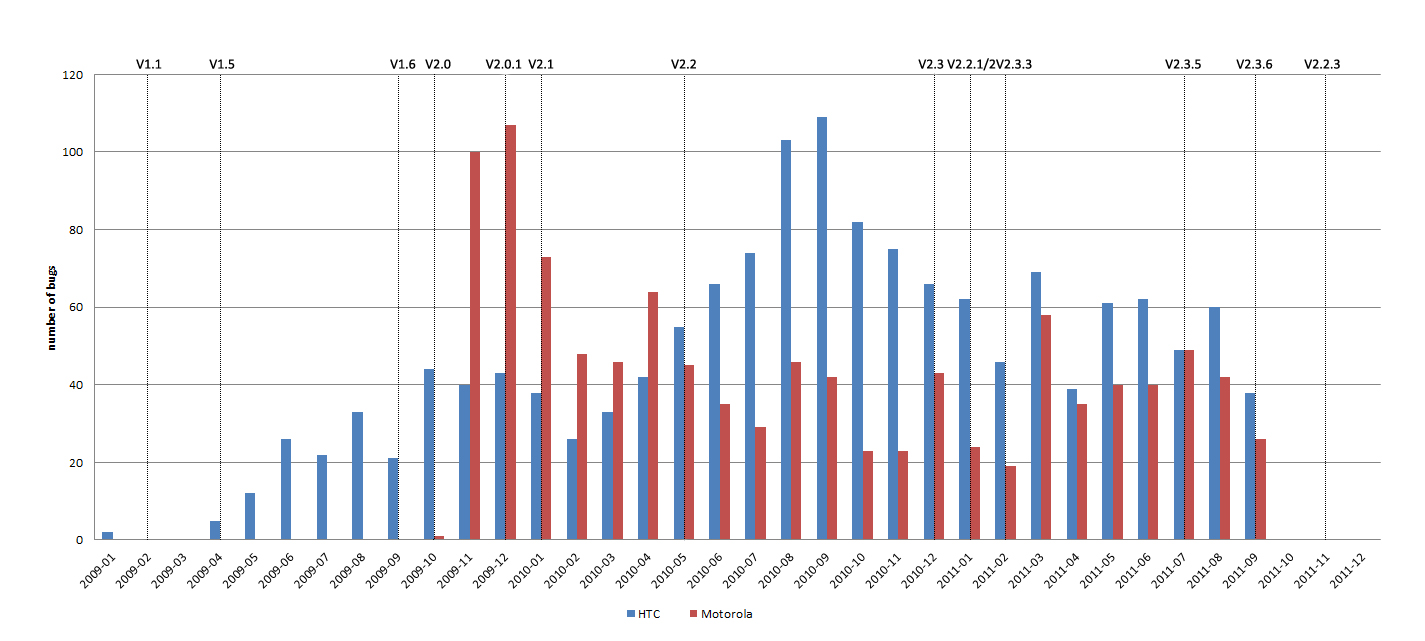
\includegraphics[width=1\textwidth]{bugovertime.png}
%\caption{Number of bugs with the major version of Android for HTC and Motorola}
%\end{figure*}



\section{Related Work}
Topic models have been used to help understand software systems. Marcus et al.\cite{Marcus04aninformation} used Latent Semantic Indexing (LSI) on both source code and user queries and then identified the most relevant source code documents with similarity measurements. Asuncion et al.\cite{Asuncion:2010} applied a coherence measurement on topics learned by LDA to model the quality of bug reports. Linstead et al.\cite{Linstead:2009} performed LDA to generate traceability links for artifacts in software projects automatically. Topic modeling is also utilized by Thomas et al.\cite{Thomas:2011} to study the evolution of topics in software projects.

Compared with all these approaches, our work differs from them in two aspects. We manually labeled bug reports with multiple labels. And we applied labeled LDA in our work to overcome the disadvantages of these unsupervised algorithms by pre-defining the number of topics and interpreting the extracted topics \cite{Asuncion:2010}.

\section{Methodology}

Our methodology is to extract bug reports, assign multiple labels to
each of them and then perform Labeled LDA on the labeled data. 
In
order to compare the performance between LDA and Labeled LDA, we also
apply LDA on the extracted bug reports of HTC and Motorola without our
manual labels. 
We label all the topics generated by LDA. 
For each
vendor, we calculate the similarity of each pair of labels from LDA
and Labeled LDA to evaluate their performance. 
After that we calculate
the average relevance of bug reports to each label over
time\cite{Hindle} and compare them between two Android vendors, HTC
and Motorola.

\subsection{Generating the data}2

We use the Android bug reports provided by the MSR Mining Challenge
\cite{MSRChallenge2012}and store all the XML data into a SQL
Server. 
Using regexes, we extract bug reports highly related to
Android phones of HTC and Motorola respectively. 
We use the title,
opened date and description in each bug report. 
After removing all the
declined and duplicate bug reports, we have 1503 HTC bug reports and
1058 Motorola bug reports.

\begin{table}[!t]
\renewcommand{\arraystretch}{1.3}
% if using array.sty, it might be a good idea to tweak the value of
% \extrarowheight as needed to properly center the text within the cells
\caption{Selected Manual labels from bug reports of HTC and Motorola. There are at least 20 bug reports are assigned to these labels.}
\label{selected1}
\centering
\begin{tabular}{|c||l|}
\hline
Vendor & Label\\
\hline
HTC & sms\//mms browser calendar network audio contact display \\ 
  & email system Layout android\_market bluetooth wifi keyboard\\
  & synchronize setting calling language time app input image\\
  & dialing search\\
\hline
Motorola & app email audio browser display contact upgrade screen\\
    &sms\//mms calendar system calling synchronize image \\
    &GPS android\_market setting network keyboard lock Layout \\
    &notification dialing wifi bluetooth\\
\hline
\end{tabular}
\end{table}


\subsection{Multi-labeling}
We manually tag bugs with multiple labels. The labels are defined as the functionalities 
and applications on an Android mobile phone, such as SMS/MMS, browser and Wi-Fi or the components of the handsets mentioned in the bug reports, such as GPS, screen and keyboard. Most of the labels about functionalities and applications are based on the detailed introduction to the features, specifications and applications of Android operating system\footnote{\url{http://en.wikipedia.org/wiki/Android_operating_system}}. The labels about components of the handsets are mostly extracted from the description of comparison of Android devices\footnote{\url{http://en.wikipedia.org/wiki/Comparison_of_Android_devices}}.

First, two of us (Zhang and Fan) separately tag the HTC 248 bug reports in 2009 with the multiple labels. Then we train each author’s labeled data with STMT. By comparing each set of trained topics in the results and returning to the bug reports, we check to ensure the same interpretation of each bug when labeling. Then we come up with the same labeling rules to process the data. After this, we tag the rest of bug reports separately for both HTC and Motorola. When there is a bug report that cannot be tagged by the labels we already have, we would create a new label together based on our definition of labels, i.e. the functionalities and applications on an Android mobile phone or the components of the handsets. For example, the label ``calculator'' is created by this way. At first we could not expect this basic application on mobile phones would have bugs. However, there are several bugs that complained the correctness of the calculator's results. So we added it to our labels. The manual labeling took approximately 30 hours per person. In the end, for HTC and Motorola there are 199 and 73 bug reports that cannot be labeled respectively. We have tagged 1304 HTC and 985 Motorola bug reports, each with multiple labels. In total, there are 72 labels for HTC and 57 labels for Motorola. Table \ref{selected1} selects Manual labels from bug reports of HTC and Motorola. There are at least 20 bug reports are assigned to these labels.

\subsection{Applying Labeled LDA}
To apply Labeled LDA we preprocessed the labeled bug reports. We convert the title and description of each bug report to lowercase and remove stop words (words that are less than 3 characters and common English stop words such as ``all'', ``about'', ``the'', ``that'' and ``were'' ).
By applying Labeled LDA to the bug reports of HTC and Motorola separately, we have the word distribution of each label and a matrix that provides the relationship between bug reports and the labels. The topic analysis is based on these results. In order to investigate the trend of each label by time, we grouped all the bug reports by month from 2009 to 2011 based on their open date for each of the two vendors. For each label, we computed the average relevance values of bug reports to this label in each month. The average relevance value of a label \begin{math} \l_i \end{math} in month \begin{math} m_j \end{math} is the sum of all the relevance values of this label over all bug reports in this month divided by the number of bug reports in this month,
\begin{equation}
A(\l_i,m_j) = \frac{\sum_{\substack{k=1}}^{|m_j|}r(\l_i,d_k)}{|m_j|}
\end{equation}
where $r(\l_i,d_k)$ is the relevance value of label $\l_i$ to bug report $d_k$, $|m_j|$ is the number of bug reports in this month. This metric is to sum all the relevance values. At last we generated a distribution of average relevance among 36 months for each label.

\subsection{Applying LDA}
In order to compare the performance between LDA and Labeled LDA, we also apply LDA on the extracted bug reports of HTC and Motorola without our manual labels. We used the same preprocessing method on the HTC bug reports when applying LDA. 

To choose the number of topics $n$, we ran LDA using multiple values of $n$ that included: 10, 15, 20, 25, 30, 35, 40, 45, 50, 55, 60, 65 and 70 on the bug reports of HTC. Three of the authors evaluated the word distribution of each topic together in each case. We then chose the $n$ is equal to 35 where the topics generated by LDA were distinct enough from each other, had few repetitions and could be interpreted well by the authors. Other researchers had some similar results \cite{Thomas:2011} \cite{Hindle}. We did the same process on the bug reports of Motorola and we chose the number of topics is equal to 30. We also labeled each topics generated by LDA for both vendors and the labels are based on our manual labels. Three of the authors annotated the topics together and it took two hours in total to finish all the labeling work. Table \ref{seleted2} lists a few selected topics from LDA with manual labels.


\subsection{LDA vs. Labeled LDA}
Both of the results from LDA and Labeled LDA are the matrices that provide the relationship between bug reports of two vendors and the labels. We want to explore whether LDA would generate the similar results to Labeled LDA. That is if the topics generated by LDA that were labeled as the same ones in Labeled LDA would be related to similar bug reports.
The Jaccard similarity coefficient is applied to compute the similarity between each topic in LDA and each label in Labeled LDA. That is, the Jaccard similarity coefficient between label A in LDA and label B in Labeled LDA is the ratio of the intersection of bug reports related to label A and label B to the union of the bug reports related to label A and label B,
\begin{equation}
sim(A,B) = \frac{\phi(A,d)\bigcap\phi(B,d)}{\phi(A,d)\bigcup\phi(B,d)}
\end{equation}
where the $\phi(A,d)$ is the set of bug reports that has relevance values to label A and $d$ is a set of all the bug reports in each vendor.

We used several thresholds (0.01, 0.05, 0.1, 0.2, 0.3, 0.4 and 0.5) on the relevance value of a bug report to a label in LDA when generating the Jaccard similarity coefficient and found that under the threshold is 0.2 the result is best.

\begin{table}[!t]
\renewcommand{\arraystretch}{1.3}
% if using array.sty, it might be a good idea to tweak the value of
% \extrarowheight as needed to properly center the text within the cells
\caption{Selected topics from LDA with manual labels. Word lists are inferred by LDA.}
\label{seleted2}
\centering
\begin{tabular}{|c||c||l|}
\hline
Vendor & Label & Top 10 terms\\
\hline
HTC & sms\//mms &sms, message, text, sent, send, conversation, \\
            && received, reply, time, number \\ \cline{2-3}
  & email & Email, mail, gmail, app. Inbox, send, emails, \\
            &&message, client, read \\ \cline{2-3}
  & browser&browser, page, web, http, open, website, \\
            &&webview, click, url, load\\
\hline
Motorola & wifi &connect, xoom, hotspot, netbook, wifi, ssid, \\
           &&radio, connection, feature, model\\ \cline{2-3}
    &calendar& calendar, event, sync, appointment, date, google, \\
           &&time, droid, day, change \\ \cline{2-3}
    &contact & contact, google, number, address, list, facebook, \\
           &&droid, account, sync, separate \\
\hline
\end{tabular}
\end{table}


\section{Performance of LDA and Labeled LDA}
We investigate the performance between LDA and Labeled LDA in this section.

From these two similarity plots(Figure \ref{similarityhtc} and Figure \ref{similaritymoto}) of labels between LDA and Labeled LDA, we can observe that most of the topic-label similarity values are quite small except the diagonal ones, especially in HTC. This observation is expected since most of the diagonal spots are the Jaccard similarities between the same labels from LDA and Labeled LDA. Then we counted the number of bugs that are related to labels which are both shared by LDA and Labeled LDA. That is showed by Figure \ref{bughtc} and Figure \ref{bugmoto}.

\begin{figure*}[htb]
\centering
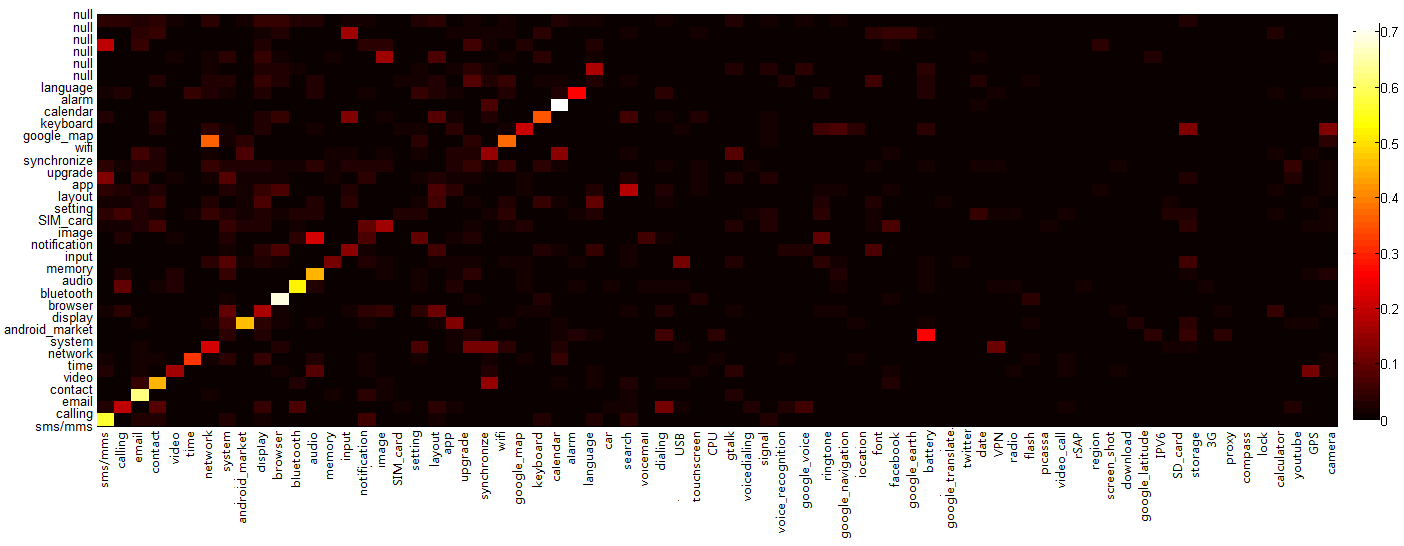
\includegraphics[width=1\textwidth]{htcsim.png}
\caption{Similarity of labels between LDA and Labeled LDA in HTC. X axis is the labels in Labeled LDA and Y axis is the labels of topics generated by LDA. The result is based on the HTC bug reports. Brighter means higher similarity.}
\label{similarityhtc}
\end{figure*}

\begin{figure*}[htb]
\centering
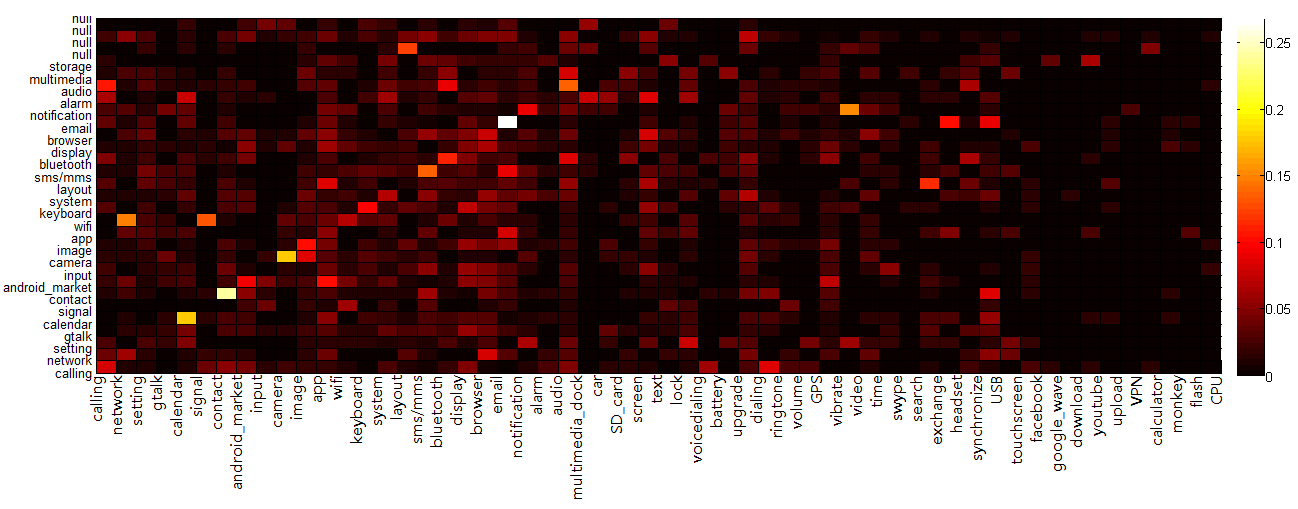
\includegraphics[width=1\textwidth]{motosim.png}
\caption{Similarity of labels between LDA and Labeled LDA in Motorola. X axis is the labels in Labeled LDA and Y axis is the labels of topics generated in LDA. The result is based on the Motorola bug reports. Brighter means higher similarity.}
\label{similaritymoto}
\end{figure*}

Most of the same labels from LDA and Labeled LDA have the comparable amount of bug reports. For example, the label ``calling'' from the HTC bug reports has exactly the same number of bugs related to for both results of LDA and Labeled LDA. However, the similarity of these related bug reports in terms of this label ``calling'' is very low which means LDA and Labeled LDA related quite different bug reports to this label. When doing this comparison, we cannot ignore the number of bugs that related to each label from both two techniques. That is, for one label, the ratio (the smaller number is divided by the bigger number so the ratio is always less or equal to one) of the number of bug reports related to this label predicted by LDA to that of Labeled LDA would be the upper bound of the similarity value. From Figure \ref{bughtc} and Figure \ref{bugmoto} that the relation between topics and each bug report modeled by LDA is quite different from the results generated by Labeled LDA.

The similarity values for these labels in Figure \ref{similaritymoto} are quite low compared with the ratio. Only about ten labels in HTC have similarity values that are larger than half of the ratio. For Motorola, the similarity values are all very low compared with the upper bound of the similarity values.

From all above, we can conclude that only a few of the bug reports in HTC and Motorola are predicted by LDA and Labeled LDA to be related to the same labels. In other words, the relation between topics and each bug report modeled by LDA is quite different from the results generated by Labeled LDA. We think the manual efforts of labeling all the bug reports would help us gain the better topic models generated by Labeled LDA. 
\begin{figure}[htb]
\centering
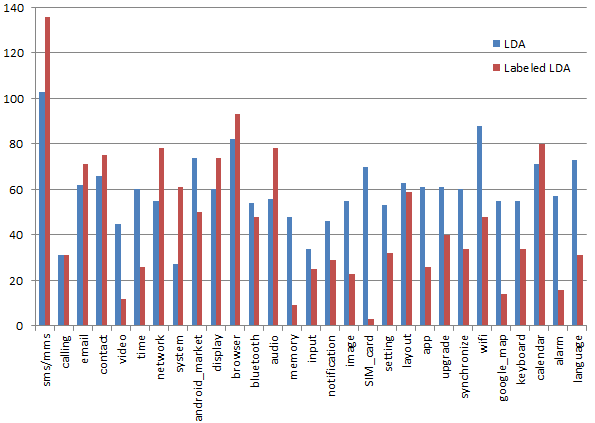
\includegraphics[width=0.5\textwidth]{htcldallda.png}
\caption{Comparison of number of bug reports related to the same labels from LDA and Labeled LDA in HTC. The X axis is the same labels from LDA and Labeled LDA and the Y axis is the number of bug reports.}
\label{bughtc}
\end{figure}
\begin{figure}[!htb]
\centering
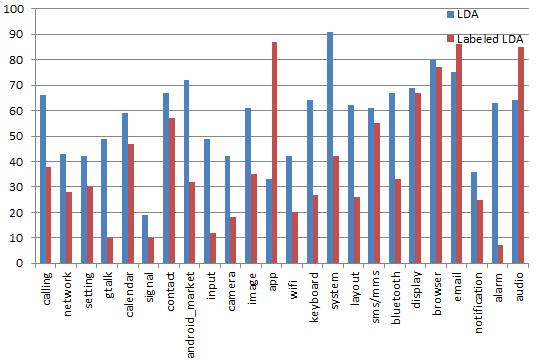
\includegraphics[width=0.5\textwidth]{motoldallda.png}
\caption{Comparison of number of bug reports related to the same labels from LDA and Labeled LDA in Motorola. The X axis is the same labels from LDA and Labeled LDA and the Y axis is the number of bug reports.}
\label{bugmoto}
\end{figure}
Hence we chose to use the Labeled LDA to do topic analysis in the following sections.

\begin{figure}[htb]
\centering
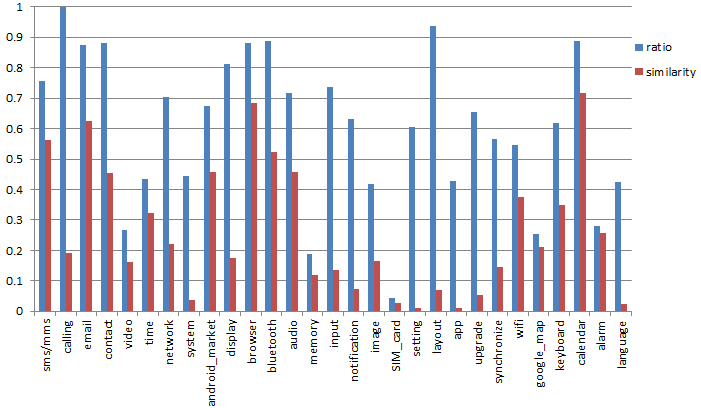
\includegraphics[width=0.5\textwidth]{htcratiosim.png}
\caption{The comparison of ratio and similarity in HTC. The result of the smaller number of bug reports related to this label in LDA or Labeled LDA divided by the larger one is the ratio of this label. The X axis is the same labels from LDA and Labeled LDA.}
\end{figure}

\begin{figure}[htb]
\centering
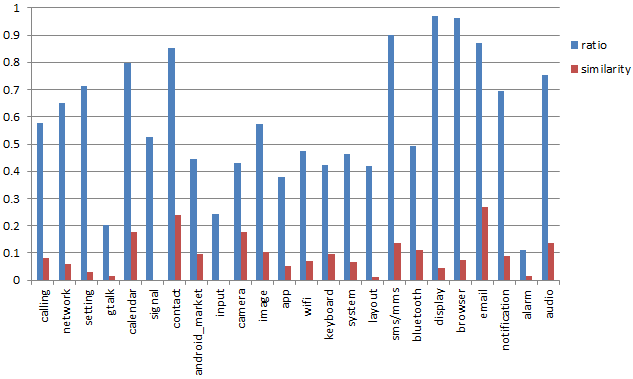
\includegraphics[width=0.5\textwidth]{motoratiosim.png}
\caption{The comparison of ratio and similarity in Motorola. The result of the smaller number of bug reports related to this label in LDA or Labeled LDA divided by the larger one is the ratio of this label. The X axis is the same labels from LDA and Labeled LDA.}
\end{figure}


\section{Topic Mining and Analysis}

In order to investigate fragmentation within Android, we mined the bug report of Android System and analyzed the result from both quantity and quality views. 

We start by exploring the quantity of bug reports for HTC and Motorola. Then we compare and discuss the topic relevance over time for both vendors.

%\begin{figure}[!htb]
%\centering
%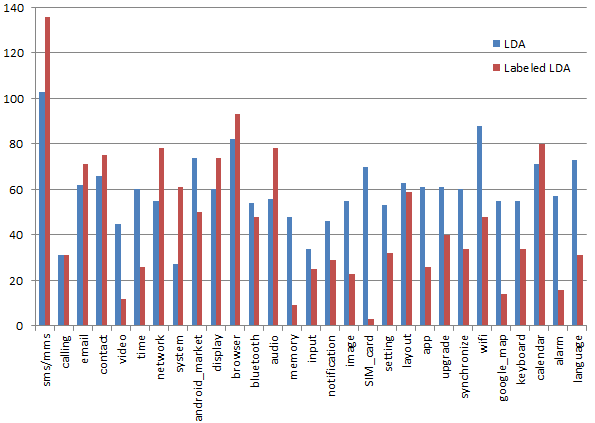
\includegraphics[width=0.4\textwidth]{htcldallda.png}
%\caption{Comparison of number of bug reports related to the same labels from LDA and Labeled LDA in HTC. The X axis is the same labels from LDA and Labeled LDA and the Y axis is the number of bug reports.}
%\end{figure}
%
%\begin{figure}[!htb]
%\centering
%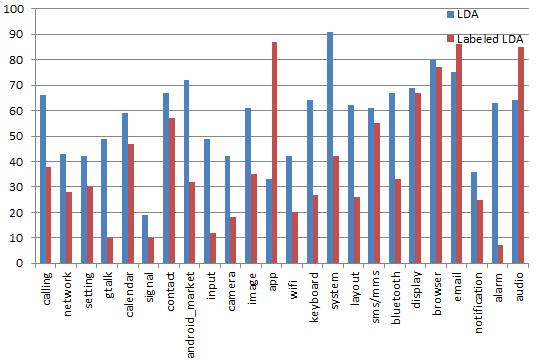
\includegraphics[width=0.4\textwidth]{motoldallda.png}
%\caption{Comparison of number of bug reports related to the same labels from LDA and Labeled LDA in Motorola. The X axis is the same labels from LDA and Labeled LDA and the Y axis is the number of bug reports.}
%\end{figure}
%
%\begin{figure}[htb]
%\centering
%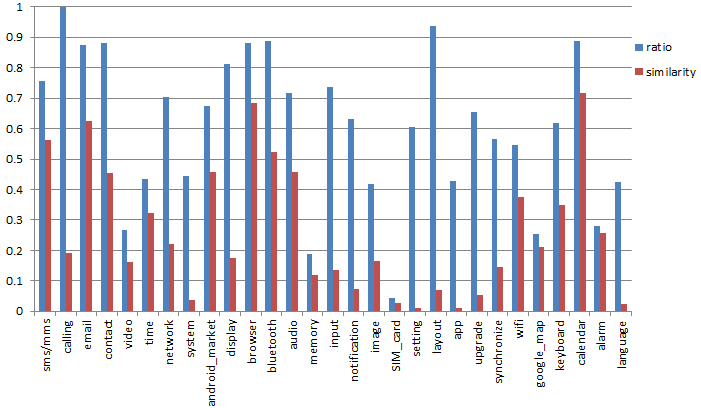
\includegraphics[width=0.4\textwidth]{htcratiosim.png}
%\caption{The comparison of ratio and similarity in HTC. The result of the smaller number of bug reports related to this label in LDA or Labeled LDA divided by the larger one is the ratio of this label. The X axis is the same labels from LDA and Labeled LDA.}
%\end{figure}
%
%\begin{figure}[htb]
%\centering
%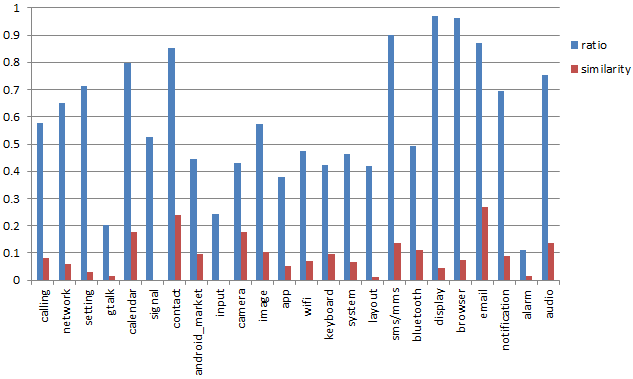
\includegraphics[width=0.4\textwidth]{motoratiosim.png}
%\caption{The comparison of ratio and similarity in Motorola. The result of the smaller number of bug reports related to this label in LDA or Labeled LDA divided by the larger one is the ratio of this label. The X axis is the same labels from LDA and Labeled LDA.}
%\end{figure}

\subsection{Overview of bug reports in HTC and Motorola}

We group the bugs monthly based on their opened date and count the total number of bugs in each month for two vendors. Figure \ref{bugovertime} depicts a comparison of the quantity of bugs for HTC and Motorola.

Figure\ref{bugovertime} shows the first HTC bug report was opened in January, 2009, and the first Motorola bug report was opened in November, 2009. According to the brief history of Android phone survey\cite{historyofandroid}, HTC released the first Android phone in October, 2008, while Motorola releases the first phone in October, 2009. The first bug reports of both vendors are in order of the first phone released by them. 

In addition, we can see, in Figure1, the spike for HTC is in September, 2010, and that for Motorola is in December, 2009. By reading the bug subjects, we found that the HTC spike is because many people upgrade Android 2.1 to Android 2.2. The Motorola spike is mainly because the upgrade from Android 2.0 to Android 2.0.1. This suggests that bug activity increases are more relevant to Android version than hardware platform.  

\begin{figure*}[htb]
\centering
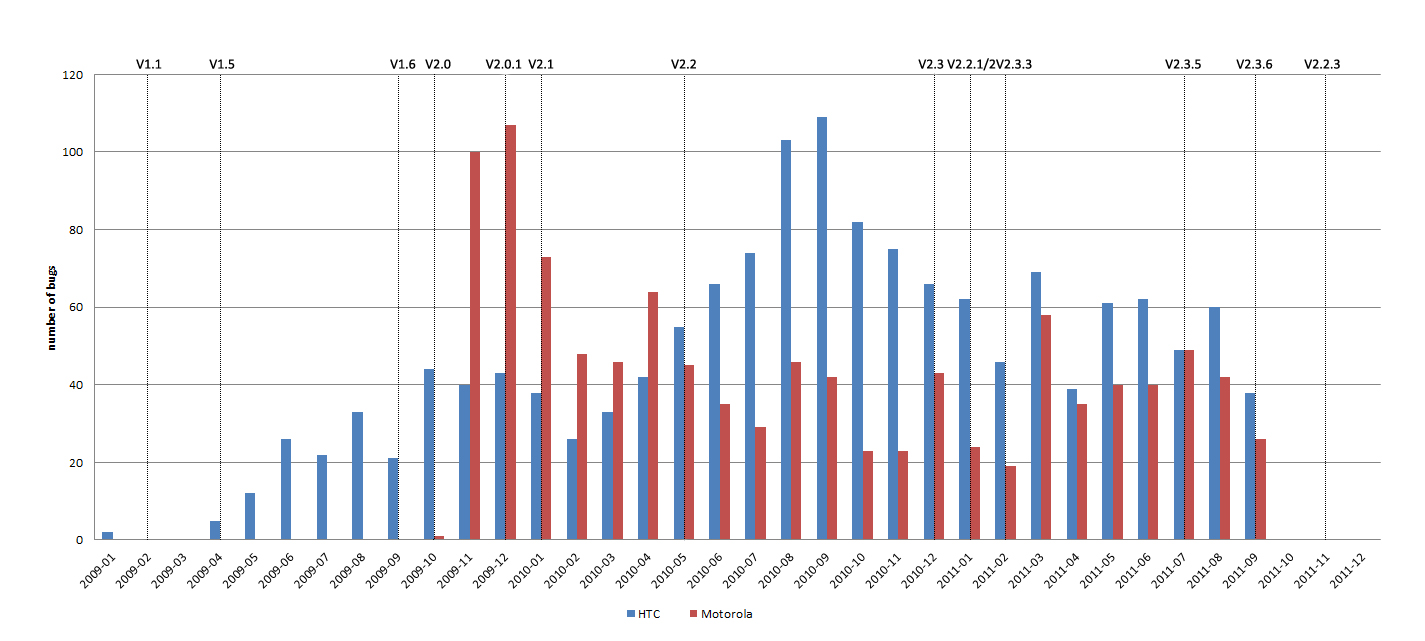
\includegraphics[width=1\textwidth]{bugovertime.png}
\caption{Number of bugs with the major version of Android for HTC and Motorola}
\label{bugovertime}
\end{figure*}


\subsection{Topics Analysis of HTC and Motorola}

First, it should be mentioned that we extracted 72 topics for HTC and 58 topics for Motorola with Labeled LDA.

By calculating the average of bug distributions associated with the topic, we got the average relevance for each topic by month. Examining the average relevance trends for each topic and comparing them for both vendors, we categorize the topics into three types. They are common troubled topics, common improved topics, and unique topics. The Common Troubled Topics mean that the relevance of topic has fluctuations all the time for both HTC and Motorola. The Common Improved Topics mean that the relevance of topic turns to be flat after several fluctuations over time for HTC and Motorola. The Unique Topics mean that the relevance of topic has significant differences between HTC and Motorola.

A representative subset of top 18 topics, which are obtained by sorting the number of related bug reports for HTC and Motorola respectively, is given in Table\ref{topicslist}, Table\ref{topicslist} and Table\ref{topicslist} [THE TABLEIII SHOULD BE SPLIETED INTO THREE TABLES]. Table\ref{topicslist} shows Common Troubled Topics, Table\ref{topicslist} shows Common Improved Topics, and Table\ref{topicslist} shows Unique Topics. Each topic is described by top 15 terms associated with the topic for both HTC and Motorola. These topics are associated with 85\% bugs of HTC, and 83\% bugs of Motorola. In Table\ref{topicslist}, Table\ref{topicslist} and Table\ref{topicslist}, the label column represents the features of Android as mentioned before.

\begin{figure*}[htb]
\centering
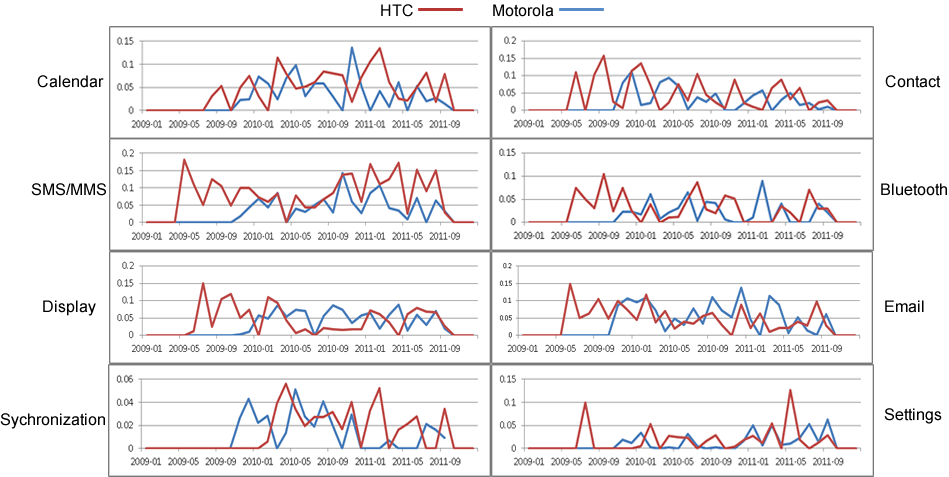
\includegraphics[width=1\textwidth]{commontopic.png}
\caption{Common Troubled Topics in HTC and Motorola}
\label{commontopic}
\end{figure*}

\subsubsection{Common Troubled Topic} 

A representative subset of eight Common Troubled Topics shared by two vendors is shown in Table1 and the average relevance of each topic is shown in Figure\ref{commontopic}. 

In Table\ref{topicslist}, HTC and Motorola share many identical terms for each label. That means they have the same issues for SMS(text, thread, send), Calendar(event, day, google,appointment,time), Email(gmail, send, thread), Contact (number, google,list), Display (screen,button,behavior), Bluetooth ( headset,connect, calling), Synchronization (contact, exchange, google) and Settings(turn,network,mode). 

We also found that multiple topics share some same terms for each vendor. For HTC, we can see, five topics including SMS/MMS, Contact, Display, Bluetooth and Settings share the same term “desire”. This indicates that these topics happened frequently for HTC Desire model. Calendar and Bluetooth share the same term “2.2” which means Android version 2.2. This indicates that these two topics happened frequently for Android 2.2 in HTC models. For Motorola, seven topics except Settings share the same term “droid” which means Motorola Droid model. In addition, Calendar and Synchronization in Motorola share “milestone” which indicates these two topics discussed mostly in Motorola Milestone model. “Xoom” shared by Display and Settings indicates that Motorola Xoom has more bugs related with these two topics. Furthermore, “Synchronization” topics include both “Xoom” and “milestone” terms. This indicates bugs related with synchronization happened frequently in both Motorola Xoom and Motorola Milestone. 

In Figure\ref{commontopic}, HTC and Motorola share the same topic evolution trends. Both of them have continuous spikes and drops for each topic over time. That indicates bugs associated with these topics have no obvious decreasing trends with Android evolution.

In summary, both of HTC and Motorola have some topics associated with their typical models. And both of HTC and Motorola have some topics associated with Android 2.1 and Android 2.2. As the topics represent features in Android, we can see there might be a compatibility issue for some topics for both vendors. 

\begin{figure*}[htb]
\centering
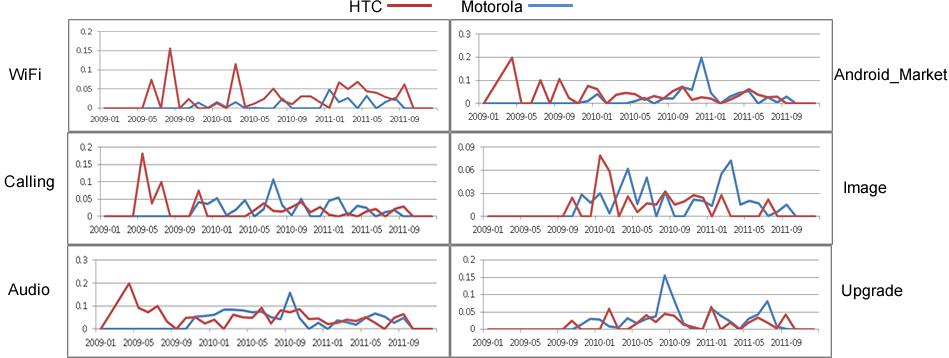
\includegraphics[width=1\textwidth]{fixtopic.png}
\caption{Common Improved Topics in HTC and Motorola}
\label{fixtopic}
\end{figure*}

\subsubsection{Common Improved Topic}

A representative subset of six Common Improved Topics shared by two vendors is shown in Table2 and the average relevance of each topic is shown in Figure\ref{fixtopic}.

In Table\ref{topicslist}, HTC and Motorola share many identical terms for WiFi (connection,ssid,network,etc), Upgrade (2.2,2.1,http), Image (gallery,picture,photo) and so on. For both of HTC and Motorola, bugs related with Upgrade happened in Android 2.1 to Android 2.2. This indicates Android 2.2 might have compatibility issue. 

In the meanwhile, they also own some special terms. For HTC, bugs related with Calling happened frequently in Android 2.1, and bugs related with Image and Audio happened frequently in Android 2.2. For Motorola, bugs related with Calling happened frequently in Android 2.2 and bugs related with Keyboard happened frequently in Android 2.0.1.

From Figure\ref{fixtopic}, we can see both HTC and Motorola have spikes in the early stage, and then stay in their values. It indicates these features tend to be more robust over time with Android evolution during the whole observed period.

In summary, both of HTC and Motorola have some topics associated with their typical models. The same topics for both vendors happed frequently in the different Android versions.

\subsubsection{Unique Topics}

There are the two unique topics for HTC shown in Table\ref{topicslist}. And Figure\ref{uniquehtc} shows the average relevance of each topic.

In Table\ref{topicslist}, only HTC has the Language (arabic, desire, language, 2.2, letters, characters, translation, character, read) topic. The associated terms indicate that bugs related with language happened frequently in Android 2.2. This stems from the fact that the keyboard multiple language function is a new function introduced in Android 2.2. Moreover, most of HTC models have no physical keyboard, so this new function has been used frequently by HTC users. In contrast, for Motorola, most of models have the physical keyboard, so this function has been used seldom. This fact can also be the reason why HTC has “on-screen” and “virtual” for keyboard, while Motorola has no these terms at all.

In figure\ref{uniquehtc}, HTC keyboard turns to stay in its value, while Motorola has spikes and drops over time. HTC language has the relevance distribution, while there are too few bugs related with language to make language as a topic in Motorola.

\begin{figure*}[htb]
\centering
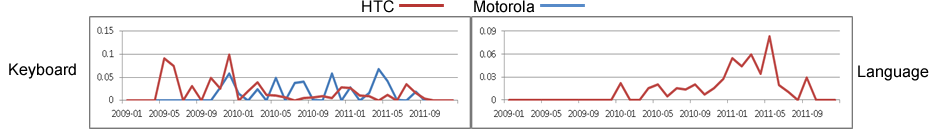
\includegraphics[width=1\textwidth]{uniquehtc.png}
\caption{Unique Topics relevance in HTC}
\label{uniquehtc}
\end{figure*}

\begin{figure*}[htb]
\centering
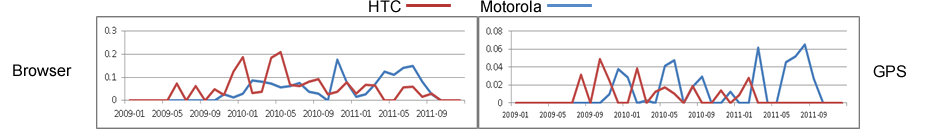
\includegraphics[width=1\textwidth]{uniquemoto.png}
\caption{Unique Topics relevance in Motorola}
\label{uniquemoto}
\end{figure*}


There are the two unique topics for Motorola shown in Table\ref{topicslist}. And Figure\ref{uniquemoto} shows the average relevance of each topic.
In Table\ref{topicslist}, HTC and Motorola, on the one hand, share the same terms for GPS (gps, data, position, location, maps, google, time, lock, wrong, icon, turn, home, latitude) and browser (Browser, page, text, http, open, server). On the other hand, they have special terms for their own. For browser, Motorola has “droid”, “milestone” and “xoom” terms together. This indicates that the browser bugs associates three Motorola models. This indicates that Browser feature has portability issue within Motorola Android models.

In figure\ref{uniquemoto}, we can see the relevance for GPS and Browser demonstrates different. For HTC, they have stripes and drops in the early stage, and then stay in their values. For Motorola, they stay in their values and then have stripes and drops afterwards.


In summary, for different vendors, the same topic show significantly different relevance as a result of the different model designs.


\section{Discussion}

[THIS PART SHOULD BE UPDATED LATER, BUT NOT FINISHED YET]

In this section, we want to discuss this question and try to give a reasonable answer based on our analysis.

\begin{table*}[!htb]
\renewcommand{\arraystretch}{1.3}
% if using array.sty, it might be a good idea to tweak the value of
% \extrarowheight as needed to properly center the text within the cells
\caption{Common Topics and associated Word List with Related Top 10 Terms}
\label{topicslist}
\centering
\begin{tabular}{|c||c||c||c|}
\hline
Topic Type & Label & HTC & Motorola\\ 
\hline
Common Troubled Topics & SMS\//MMS &message,	sms,	text, thread, time,  & message, text, sms, droid, send,	\\
%&& sent, desire, contact, new, number, &	thread, messaging, sent,user, version, issue, \\ 
&&conversation, send, version, app, screen &thread, person, threads, number, http\\ \cline{2-4}

  & Email & email	, mail, gmail, app, message,   &email, droid, account,	gmail, mail, \\
            %&&inbox, messages,client,emails, account,  &server, message,	user,	emails, exchange, \\ 
            &&send, interface, thread, time, new & file, version, open, device, app\\ \cline{2-4}
            
  & Calendar&calendar, event, day, events, google,  &calendar,	event, droid, google, appointment, \\
%            &&view, 2.2,time,month, date, version, &events, day, field, date, appointments, \\ 
            &&reminder, appointment,  edit, running &outlook, milestone, data, app, version\\ \cline{2-4}
            
  & Contact & contact, contacts, number, freed, activity,  &contact, contacts, droid, number, numbers, \\
%            &&displayed, list, group, google, numbers,   &address, version, google, menu, correct, \\
            &&starting,desire, user, version, field & behavior, different,list, option, gmail\\ \cline{2-4}
            
  & Display\//Screen&screen, version, desire,	behavior, app, &droid, screen, button, correct, home, \\
%   && number,code, final, press, sure, &display, behavior,  landscape, 2.1,  menu	, \\
   &&home,user, black, new,	power  &bar, xoom	,device, user, status\\ \cline{2-4}
   
  & Bluetooth & bluetooth,headset, car, connect, device,  &bluetooth,	headset, droid, device,connected, \\
%            &&connection, version, data, app, desire &connect, devices, calls,car,	issue, \\
            &&desire,	2.2, work, connects, behavior,2.1 &connection, 2.2, car,pair, time\\ \cline{2-4}
            
  & Synchronization&contacts, account, sync, exchange, contact, &sync, google, account, contacts, device, \\
%            &&Google, ears, device, group, server, &contact, group, time, exchange, contactsq"e, \\
            &&Gmail, policy, new, list, display&display, groups,  list,  droid, milestone\\ \cline{2-4}
            
  & Setting&Volume, sound,	set, pattern,  default,&Settings, device, menu, turn,	network, \\
%            && Turn, desire, static, control, apps,&vpn, honeycomb, button, xoom,  settings-q, \\
            && change, settings, media, dns, screen &behavior,	right, wireless, headset, mode\\
\hline

Common Improved Topics & Keyboard &keyboard, input,	text, key,number,&keyboard, droid, keys,text, press, \\
           && on-screen, mode, field,
landscape,virtual &space, box, open, device,landscape\\ \cline{2-4}
           
    &Browser& page, text, http, open, server,&droid, page, web, http, open, \\
           && version, desire, client, 2.1, button  &xoom, html, behavior, milestone, 3.1 \\ \cline{2-4}
           
               &Audio& music, audio, player, file, play, &music, droid, player, media, audio,  \\
           &&2.2,sound, playback,reproduce, mp3 &files, volume, play, running, genre\\ \cline{2-4}
           
               &Calling& number, calls, calling, 2.1, receive, &droid, calls, number, button, answer,  \\
           && called, button, answer, bluetooth, desire,  &incoming, screen, voice, speaker, 2.2 \\ \cline{2-4}
           
               &Android Market& market, app, google, account, download, &market, apps, app, device, application,  \\
           &&update, application, user, apps,	paid &update, download, purchase, google,  milestone \\ \cline{2-4}
           
    &Image & image, gallery, picture, matrix, photo,  &image, droid, wallpaper, gallery, photo,\\
           &&camera, pictures, version, 2.2, photo& picture, device,	file, select,video\\

\hline
HTC Unique Topics & Language &arabic, desire, letters, characters, translation, & NONE\\
           &&rcharacter, read, support, sms, hebrew & \\ \cline{2-4}
    &WiFi & wifi, access, network, connection, connect, &wifi, xoom, connect, hotspot, turn, \\
           &&router, ssid, desire, http, scan&connection, ssid, radio, signal, hotspots\\
\hline
Motorola Unique Topics & GPS &gps, data, position, location, maps, &maps, gps, google, app, droid, \\
           &&google, time,lock, latitude, unit &location, navigation, map,traffic,update,\\ \cline{2-4}

    &Upgrade & gps, data, position, location, maps, &update, droid, 2.1,2.2, home, \\
           &&google, time, lock, wrong,tag&http,longer, settings, performance\\
\hline
\end{tabular}
\end{table*}




\subsection{Does Android have fragmentation issues?}

In this paper, the fragmentation of Android system involved in the bug reports are Android 1.x, 2.x and branches of Android systems on multiple devices in HTC and Motorola. 

According to the analysis result, common troubled topics existing in both HTC and Motorola Android device indicates that no matter how different the Android system is and how different the device is, the topics turns to be up and down all the time. Common Improved topics of both HTC and Motorola indicate that the problems were caused by the fragmentation of Android system with different versions and that of Android system from branches of both vendors. Unique topics for HTC and Motorola indicate that the bugs were caused by the branches of Android system from vendors.

Besides the three topics, upgrade bugs in both vendors can also be an evidence of fragmentation issues. Before upgrading Android system on devices, each vendor should evolve their own branch of Android system based on the combination of the original version on that device and the latest Android system. The bugs that some functions did not work after upgrade could be eliminate by one piece of maintenance of Android system. 

Therefore, we can conclude that Android system has fragmentation issues.

\subsection{Who can benefit from the Topic analysis?}

In this paper, the topic analysis suggests the robust and evolution of functions in Android system on devices from different vendors. The analysis result can be used by different people.
	
For Android system community, the findings enable them to find out which functions have severe problems, which functions have fewer problems, and which functions correlated with each other have more problems. It can also make them to distinguish problems of vendors from others. In addition, the clear idea about the problems of vendors makes community to realize what should be documented and emphasized in corresponding documentations. The concrete and detailed documentation can help reduce the chance of fragmentation issues.

For stakeholders, the findings make them have a whole picture about the function robust of their devices. In the meanwhile, they can also get information about other vendors. With the comparison of the same topics between two vendors, other vendors can easily get some lessons learn which guide them during design and customizing their own system.

For developers, the findings make them know how robust these functions would be. Furthermore, combining correlation among different functions in the code level and the functions trends from bug reports, they can easily find out what functions have potential bugs.

\section{Threats to validity}

Data validity – Our data originated from MSR Mining Challenge \cite{MSRChallenge2012} and the dataset only ranges from January, 2009 to September, 2011. In addition, we extracted the bug report of HTC and Motorola with regular expression, which cannot ensure 100\% correctness extraction. 

Reliability – During labeling the bug reports, every annotator followed the same protocol and used the same labels. However, there were only two annotators working on the labeling work. The annotation could be biased considering the few number of annotators and the limited knowledge we would have.	

Analysis validity - The lack of information about the various devices for two vendors in bug reports makes it difficult to analyze the fragmentation of Android system on various devices for vendors. The analysis in this paper mainly focuses on the fragmentation of various Android systems and main fragmentation for each vendor.


\section{Conclusion and Future Work}

In this paper we studied the Android bug reports for two Android vendors, HTC and Motorola. We applied Labeled LDA and topic analysis on a corpus of manually tagged bug reports with multiple labels. Our results show that Android system has some fragmentation issues. These findings can be used by Android system community, stakeholders, Android device vendors and developers to make project dashboards, process investigation and feature analysis.

For the future work, we will plan to investigate more vendors in order to reveal vendor specific bug topics and get more concrete fragmentation issues analysis.


%\subsubsection{Multi-labeling}
%Subsubsection text here.


%\begin{figure}[htb]
%\centering
%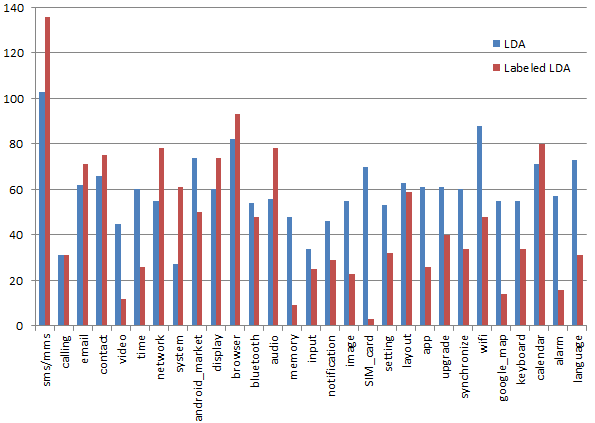
\includegraphics[width=0.4\textwidth]{htcldallda.png}
%\caption{Comparison of number of bug reports related to the same labels from LDA and Labeled LDA in HTC. The X axis is the same labels from LDA and Labeled LDA and the Y axis is the number of bug reports.}
%\end{figure}
%
%\begin{figure}[htb]
%\centering
%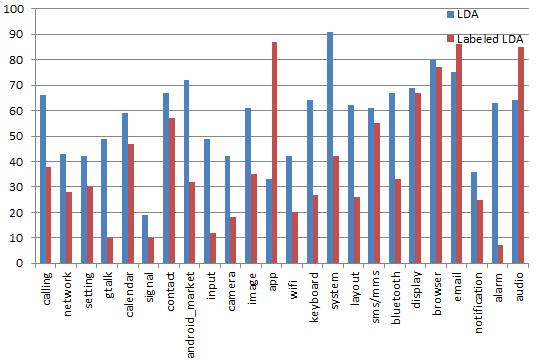
\includegraphics[width=0.4\textwidth]{motoldallda.png}
%\caption{Comparison of number of bug reports related to the same labels from LDA and Labeled LDA in Motorola. The X axis is the same labels from LDA and Labeled LDA and the Y axis is the number of bug reports.}
%\end{figure}
%
%\begin{figure}[htb]
%\centering
%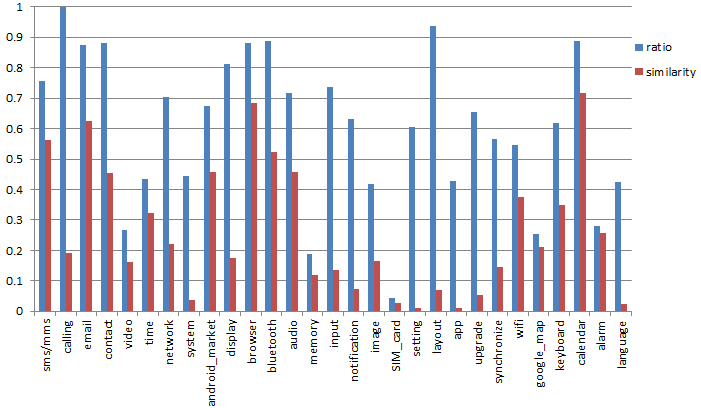
\includegraphics[width=0.4\textwidth]{htcratiosim.png}
%\caption{The comparison of ratio and similarity in HTC. The result of the smaller number of bug reports related to this label in LDA or Labeled LDA divided by the larger one is the ratio of this label. The X axis is the same labels from LDA and Labeled LDA.}
%\end{figure}
%
%\begin{figure}[htb]
%\centering
%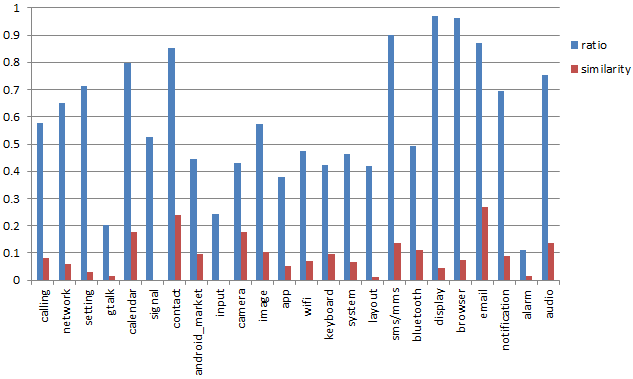
\includegraphics[width=0.4\textwidth]{motoratiosim.png}
%\caption{The comparison of ratio and similarity in Motorola. The result of the smaller number of bug reports related to this label in LDA or Labeled LDA divided by the larger one is the ratio of this label. The X axis is the same labels from LDA and Labeled LDA.}
%\end{figure}

% An example of a floating figure using the graphicx package.
% Note that \label must occur AFTER (or within) \caption.
% For figures, \caption should occur after the \includegraphics.
% Note that IEEEtran v1.7 and later has special internal code that
% is designed to preserve the operation of \label within \caption
% even when the captionsoff option is in effect. However, because
% of issues like this, it may be the safest practice to put all your
% \label just after \caption rather than within \caption{}.
%
% Reminder: the "draftcls" or "draftclsnofoot", not "draft", class
% option should be used if it is desired that the figures are to be
% displayed while in draft mode.
%
%\begin{figure}[!t]
%\centering
%\includegraphics[width=2.5in]{myfigure}
% where an .eps filename suffix will be assumed under latex, 
% and a .pdf suffix will be assumed for pdflatex; or what has been declared
% via \DeclareGraphicsExtensions.
%\caption{Simulation Results}
%\label{fig_sim}
%\end{figure}

% Note that IEEE typically puts floats only at the top, even when this
% results in a large percentage of a column being occupied by floats.


% An example of a double column floating figure using two subfigures.
% (The subfig.sty package must be loaded for this to work.)
% The subfigure \label commands are set within each subfloat command, the
% \label for the overall figure must come after \caption.
% \hfil must be used as a separator to get equal spacing.
% The subfigure.sty package works much the same way, except \subfigure is
% used instead of \subfloat.
%
%\begin{figure*}[!t]
%\centerline{\subfloat[Case I]\includegraphics[width=2.5in]{subfigcase1}%
%\label{fig_first_case}}
%\hfil
%\subfloat[Case II]{\includegraphics[width=2.5in]{subfigcase2}%
%\label{fig_second_case}}}
%\caption{Simulation results}
%\label{fig_sim}
%\end{figure*}
%
% Note that often IEEE papers with subfigures do not employ subfigure
% captions (using the optional argument to \subfloat), but instead will
% reference/describe all of them (a), (b), etc., within the main caption.


% An example of a floating table. Note that, for IEEE style tables, the 
% \caption command should come BEFORE the table. Table text will default to
% \footnotesize as IEEE normally uses this smaller font for tables.
% The \label must come after \caption as always.
%
%\begin{table}[!t]
%% increase table row spacing, adjust to taste
%\renewcommand{\arraystretch}{1.3}
%% if using array.sty, it might be a good idea to tweak the value of
%% \extrarowheight as needed to properly center the text within the cells
%\caption{An Example of a Table}
%\label{table_example}
%\centering
%% Some packages, such as MDW tools, offer better commands for making tables
%% than the plain LaTeX2e tabular which is used here.
%\begin{tabular}{|c||c|}
%\hline
%One & Two\\
%\hline
%Three & Four\\
%\hline
%\end{tabular}
%\end{table}


% Note that IEEE does not put floats in the very first column - or typically
% anywhere on the first page for that matter. Also, in-text middle ("here")
% positioning is not used. Most IEEE journals/conferences use top floats
% exclusively. Note that, LaTeX2e, unlike IEEE journals/conferences, places
% footnotes above bottom floats. This can be corrected via the \fnbelowfloat
% command of the stfloats package.


% use section* for acknowledgement
%\section*{Acknowledgment}


% trigger a \newpage just before the given reference
% number - used to balance the columns on the last page
% adjust value as needed - may need to be readjusted if
% the document is modified later
%\IEEEtriggeratref{8}
% The "triggered" command can be changed if desired:
%\IEEEtriggercmd{\enlargethispage{-5in}}

% Better way for balancing the last page:

\balance

% references section

% can use a bibliography generated by BibTeX as a .bbl file
% BibTeX documentation can be easily obtained at:
% http://www.ctan.org/tex-archive/biblio/bibtex/contrib/doc/
% The IEEEtran BibTeX style support page is at:
% http://www.michaelshell.org/tex/ieeetran/bibtex/
%\bibliographystyle{IEEEtran}
% argument is your BibTeX string definitions and bibliography database(s)
%\bibliography{IEEEabrv,../bib/paper}
%
% <OR> manually copy in the resultant .bbl file
% set second argument of \begin to the number of references
% (used to reserve space for the reference number labels box)
%\begin{thebibliography}{1}

\bibliographystyle{IEEEtran}
\bibliography{msrreference}

%\bibitem{IEEEhowto:kopka}
%H.~Kopka and P.~W. Daly, \emph{A Guide to \LaTeX}, 3rd~ed.\hskip 1em plus
%  0.5em minus 0.4em\relax Harlow, England: Addison-Wesley, 1999.

%\end{thebibliography}




% that's all folks
\end{document}


